	\documentclass[a4paperm]{article}
%\documentclass[12pt,twocolumn]{article}

\usepackage[T2A]{fontenc}
\usepackage[utf8]{inputenc}
\usepackage[russian,english]{babel}
\usepackage{amsmath,amsthm,amssymb,stackrel}
\usepackage[affil-it]{authblk}
\usepackage{cite}
\usepackage{scrextend}
\usepackage{verbatim}
\usepackage{paralist}
\usepackage[mediumspace,mediumqspace,Grey,squaren]{SIunits}
\addtokomafont{labelinglabel}{\sffamily}
\usepackage{amsmath}
\usepackage{graphicx}
\usepackage[usenames, dvipsnames]{color}
\usepackage{multirow}
\usepackage{longtable}
\usepackage{lineno}
\usepackage{xr}
 
 
%\usepackage[none]{hyphenat} %no nyphenation

\usepackage{SIunits}
\usepackage{miller}
\usepackage[version=3]{mhchem}

\usepackage{float} %H with figures

\setlength{\parindent}{5ex}



\graphicspath{{figures/}}
%\externaldocument{supplementary/aeo_supp}

\renewcommand{\thefigure}{S\arabic{figure}}
\renewcommand{\thetable}{S\arabic{table}}



\begin{document}

%\linenumbers

\title{{\bf Supporting information} \\ \bigskip
The formation of Mg-orthocarbonate through the reaction MgCO$_3$+MgO = Mg$_2$CO$_4$ at Earth's lower mantle $P-T$ conditions}


\author[1,2]{Pavel N. Gavryushkin
   \thanks{Electronic address:\texttt{gavryushkin@igm.nsc.ru, p.gavryushkin@g.nsu.ru}; Corresponding author}}     
\author[1,2]{Dinara N. Sagatova}
\author[1]{Nursultan Sagatov}
\author[3]{Konstantin D. Litasov}

\affil[1]{Sobolev Institute of Geology and Mineralogy, Siberian Branch of Russian Academy of Sciences, prosp. acad. Koptyuga 3, 630090 Novosibirsk, Russia}
\affil[2]{Novosibirsk State University, Pirogova 2, Novosibirsk 630090, Russia}
\affil[3]{Vereshchagin Institute for High Pressure Physics RAS, 108840, Troitsk, Moscow, Russian Federation}

\date{}
\maketitle

%\linenumbers

\section*{Details of the computational methods}
%%%%%%%%%%%%%%%
\paragraph{Сrystal structure predictions.}
The crystal structure prediction calculations using USPEX were performed at 25, 50, and 100 GPa for 1-4 formula units per unit cell.
The size of the first generation in the calculations was equal to 65 structures.
60\% of the structures with the lowest enthalpy were selected after the optimization and then used for the production of the next generation.
A new generation was produced as follow: 35\% of all structures were generated by heredity, 20\% - by atomic mutation, 10\% – by lattice permutation, and 35\% – randomly.
In average 38-44 generations have been produced and relaxed at each pressure.
Using AIRSS about 4000-4200 structures were randomly generated and optimized at 50 GPa, and those with the lowest enthalpy were selected.

The total energies and forces were calculated by solving the Schr\"{o}dinger equation based on projector augmented planewave implementation of density functional theory using VASP package \cite{vasp1,vasp2}.
Exchange correlation effects were treated in the generalized gradient approximation (GGA) with Perdew-B\"{u}rke-Ernzerhof scheme \cite{pbe}.
Pseudopotentials with 2p$^6$3s$^2$(Mg\_sv), 2s$^2$2p$^2$ (C), and 2s$^2$2p$^4$ (O) electrons have been used.

In all crystal structure prediction calculations, medium-quality optimization was performed using the conjugate gradient.
The medium quality settings were as follows: plane-wave cutoff energy --- 420 eV; Monkhorst-Pack k-point sampling grid of spacing --- 0.5 \AA$^{-1}$; Gaussian smearing with parameter $\sigma$ = 0.2 eV.
The most promising predicted structures were then optimized at various pressures with higher accuracy: the cutoff energy --- 600 eV, k-point sampling grid of spacing --- 0.25 \AA$^{-1}$, and $\sigma$ = 0.1 eV.

\paragraph{Thermodynamic properties.}
Phonon dispersions and free energy calculations were performed using the Phonopy package \cite{phonopy}.
Real-space force constants were calculated using supercell method and finite-displacement method, with a 2x2x2 supercell for MgO, MgCO$_3$-$R\bar{3}c$, and Mg$_2$CO$_4$-$Pnma$, 1x1x1 for MgCO$_3$-$C$2/$m$, and 2x2x1 for Mg$_2$CO$_4$-$P$2$_1$/c.
Helmholtz free energies were computed at 8 volumes (starting from 0 GPa to 150 GPa) for MgO and MgCO$_3$-$R\bar{3}c$, at 6 volumes (50-150 GPa) for MgCO$_3$-$C$2/$m$, at 7 volumes (15-150 GPa) for Mg$_2$CO$_4$-$Pnma$, and at 7 volumes (40-150 GPa) for Mg$_2$CO$_4$-$P$2$_1$/$c$, then corrected for thermal expansion using the quasi-harmonic approximation, resulting in Gibbs free energies in both pressure regimes.
In this case, high quality settings were used: the cutoff energy --- 800 eV, k-point sampling grid of spacing --- 0.2 \AA$^{-1}$, and $\sigma$ = 0.05 eV.

\paragraph{Melting temperature.}
We perform ab intio molecular dynamic simulations to determine the melting curve using Z-method, which has been proven successful to predict melting temperature in several systems.
The pseudopotentials for Mg, C, and O were the same as in the crystal structure prediction calculations.
We used plane-wave cutoff of 450 eV, and the Brillouin zone was sampled only with the $\Gamma$ point. Simulations were performed in the NVE ensemble, using supercell of Mg$_2$CO$_4$-$Pnma$ with 224 atoms, for two volumes of 57.465 and 60.982 \AA{$^3$}/f.u.
For each volume the system was simulated for 10000-14000 steps with the time step of 1.0 fs for different initial kinetic energy in order to construct an isochoric curve T vs P.

\paragraph{Elastic properties.}
The elastic constants C$_{ij}$ were evaluated using the stress-strain method $\sigma_i=C_{ij}\epsilon_j$.
Four different strains ($\pm$0.01 and $\pm$0.02) were applied in each distortion and the resulting stress-strain values were then fitted.
Obtained elastic constants then used to calculate the elastic moduli.
In order to compute elastic moduli, we apply the Voigt–Reuss–Hill approximation \cite{hill1952,hill1963}.
In this approach, the actual effective modulus for a system is approximated by the arithmetic mean of the two well-known bounds for single-crystals according to Voigt \cite{voigt1928} and Reuss \cite{reuss1929}.
The mathematical formulation is provided below.

For MgCO$_3$-$R\bar{3}c$ :
\begin{align*}
 &B_V = \dfrac{1}{9} \big[ 2 (C_{11}+C_{12})+4C_{13}+C_{33}\big], \\
 &B_R = \frac{C^2}{M}, \\
 &B =B_{VRH} = \frac{B_V+B_R}{2}. \\
 \\
 &G_V = \frac{1}{30} (M+12C_{44}+12C_{66}), \\
 &G_R = \frac{5}{2} \bigg[ \frac{C^2C_{44}C_{66}}{3B_VC_{44}C_{66}+C^2(C_{44}+C_{66})} \bigg], \\
 &G=G_{VRH}=\frac{G_V+G_R}{2}, \\
\end{align*}
where
\begin{align*}
	&M=C_{11}+C_{12}+2C_{33}-4C^2_{13}, \\
	&C^2=(C_{11}+C_{12})C_{33}-2C^2_{13}.\\
\end{align*}

For Mg$_2$CO$_4$-$Pnma$:
\begin{align*}
 &B_V = \dfrac{1}{9} \big[ C_{11}+C_{22}+C_{33}+2(C_{12}+C_{13}+C_{23}) \big], \\
 &B_R=\Delta\big[ C_{11}(C_{22}+C_{33}-C_{23})+C_{22}(C_{33}-2C_{13})-2C_{33}C_{12} + C_{12}(2C_{23}-C_{12})\\
 &	+C_{13}(2C_{12}-C_{13})+C_{23}(2C_{13}-C_{23}) \big]^{-1} , \\
 & B=B_{VRH}=\frac{B_V+B_R}{2}. \\
 \\
 &G_V=\dfrac{1}{15}\big[ C_{11}+C_{22}+C_{33}+3(C_{44}+C_{55}+C_{66})-(C_{12}+C_{13}+C_{23}) \big], \\
 &G_R=15 \big\lbrace 4 \big[ C_{11}(C_{22}+C_{33}+C_{23}) + C_{22}(C_{33}+C_{13})+ C_{33}C_{12}-C_{12}(C_{23}+C_{12})   \\
 &-C_{13}(C_{12}+C_{13})-C_{23}(C_{13}+C_{23}) \big] / \Delta + 3 \big[ \frac{1}{C_{44}}+\frac{1}{C_{55}} + \frac{1}{C_{66}} \big] \big\rbrace^{-1} , \\
 & G=G_{VRH}= \dfrac{G_V+G_R}{2}, \\
\end{align*}
 where
 
 \begin{align*}
 	&\Delta=C_{13}(C_{12}C_{23}+C_{13}C_{22})+C_{23}(C_{12}C_{13}-C_{23}C_{11})+C_{33}(C_{11}C_{22}-C^2_{12}).
 \end{align*}
 
In the following formulas, subscript $V$ denotes the Voigt bound, $R$ denotes the Reuss bound, and $VRH$ denotes the Voigt–Reuss–Hill average.

The isotropic wave propagation velocities in the material can then be evaluated from the bulk and shear moduli and the density, $\rho$, as follows

\begin{align*}
  & V_p=\sqrt{\frac{B+\frac{4}{3}G}{\rho}},
  &V_s = \sqrt{\frac{G}{\rho}}. \\	
\end{align*}

There are many descriptions of anisotropy named the compression anisotropy (A$_B$) and the shear anisotropy (A$_G$) which represent the percentage of the bulk modulus and shear modulus, correspondingly, and the universal anisotropy index. They can be obtained as follows:

\begin{align*}
	&A_B=\frac{B_V-B_R}{B_V+B_R}, \\
	&A_G=\frac{G_V-G_R}{G_V+G_R}, \\
	&A^U=5\frac{G_V}{G_R}+\frac{B_V}{B_R}-6  .  \\
\end{align*}

If A$_B$, A$_G$, and A$^U$ are equal to zero, phase turns to isotropic crystal. A$_B$ and A$_G$ could vary from 0 to 1 (i.e from 0 to 100 \% anisotropy).


\section*{Results}


\begin{figure}[H]
	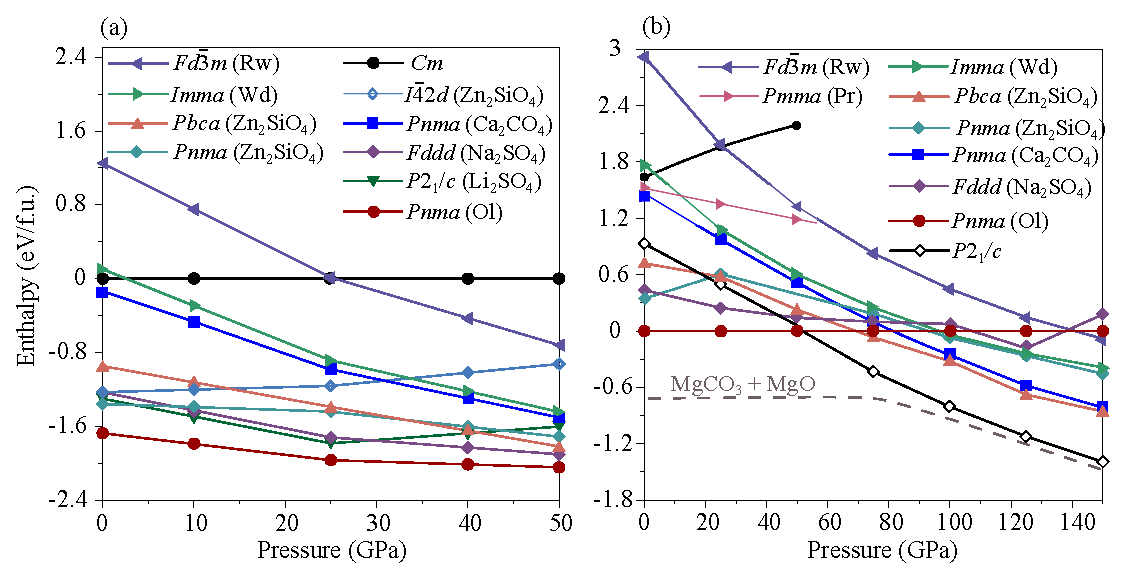
\includegraphics[width=\textwidth]{vs_Mg2CO4_for_suppl} \centering
	\caption{Enthalpy-pressure dependencies of the predicted Mg$_2$CO$_4$ structures in the pressure range 0--50 GPa (a) and 0--150 GPa (b). The grey dashed line represent relative enthalpy of the (MgCO$_3$+MgO) mixture. In legend, isostructural compounds are indicated in brackets: Rw -- ringwoodite, Wd -- wadsleyite, Pr -- poirierite, Ol -- olivine} 
\label{E-P_supp}
\end{figure}

\begin{figure}[H]
	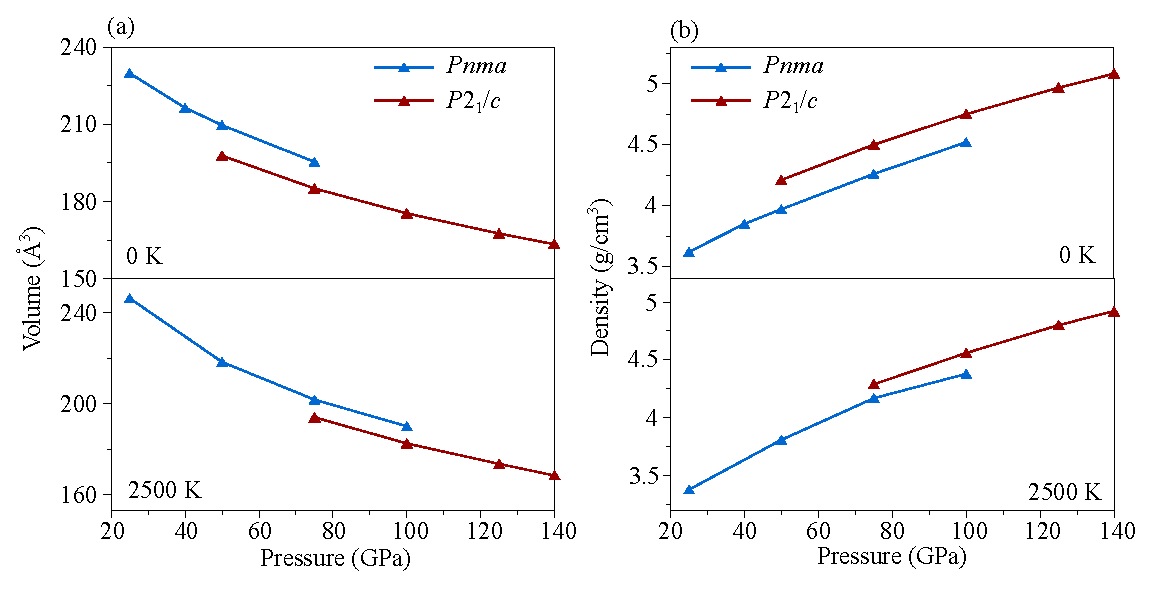
\includegraphics[width=\textwidth]{pv} \centering
	\caption{Volume (a) and density (b) dependencies of pressure for Mg-orthocarbonate.} \label{V-P}
\end{figure}

\begin{figure}[H]
	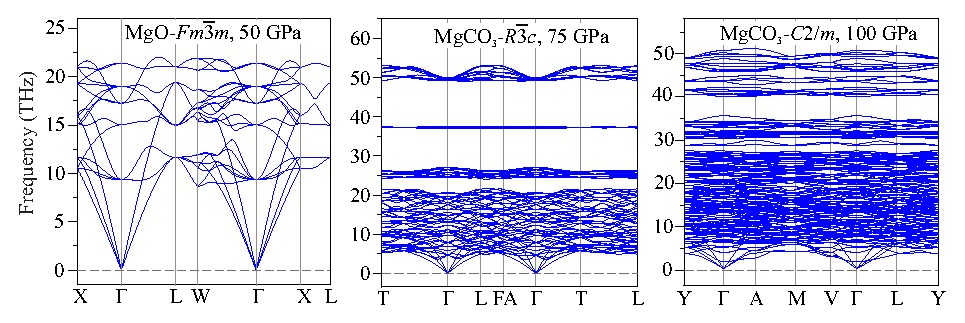
\includegraphics[width=\textwidth]{phon_MgCO3} \centering
	\caption{Phonon dispersion curves of MgO at 50 GPa, MgCO$_3$-$R\bar{3}c$ at 75 GPa, and MgCO$_3$-$C2/m$ at 100 GPa.} \label{phon_mgco3}
\end{figure}

\begin{figure}[H]
	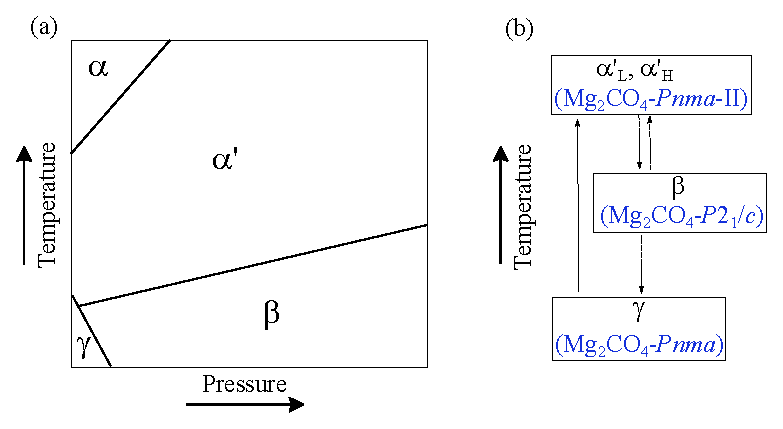
\includegraphics[width=\textwidth]{pt_scheme} \centering
	\caption{Schematic $P-T$ phase diagram of Ca$_2$SiO$_4$  according to \cite{belmonte2017} (a) and corresponding sequences of phase transitions realised on heating at ambient pressure (b). Dashed line corresponds to metastable phase transitions, solid line --- to stable transitions.} \label{ca2sio4_pt}
\end{figure}

\begin{figure}[H]
	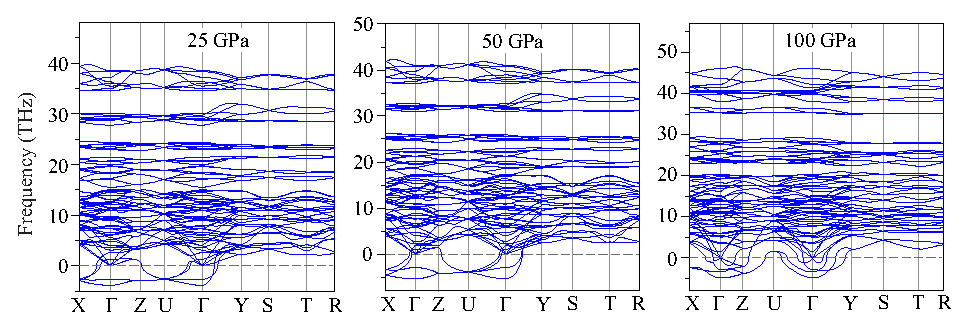
\includegraphics[width=\textwidth]{phon_Mg_Ca} \centering
	\caption{Phonon dispersion curves for dynamically unstable phase of magnesium orthocarbonate, Mg$_2$CO$_4$-Pnma-II at 25 GPa, 50 GPa, and 100 GPa.} \label{phon_PnmaII}
\end{figure}

\begin{figure}[H]
	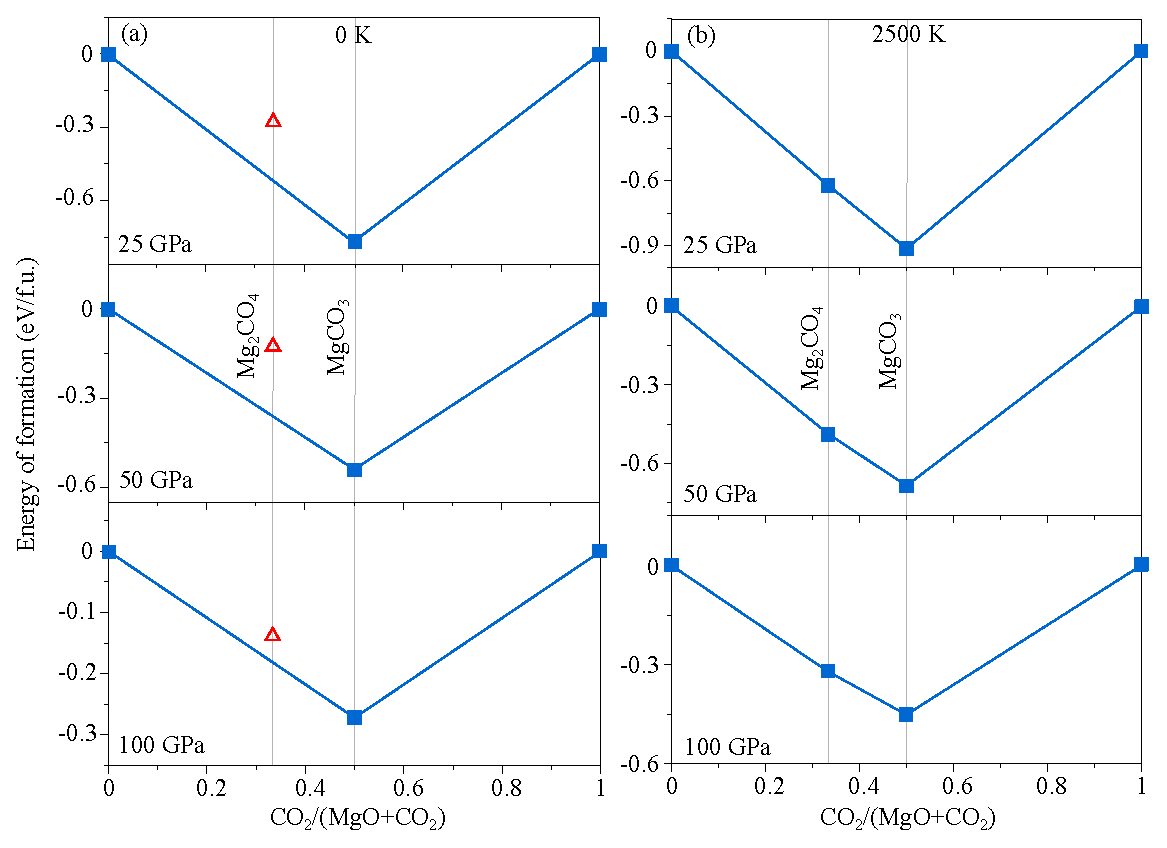
\includegraphics[width=\textwidth]{conv_hull} \centering
	\caption{Thermodynamic convex hulls for MgO-CO$_2$ system at  0 GPa, 50 GPa, and 100 GPa and 0 K (a) and 2500 K (b). Blue filled squares denote stable structures, and red open triangles --- metastable ones.} \label{conv_hull}
\end{figure}


\begin{figure}[H]
	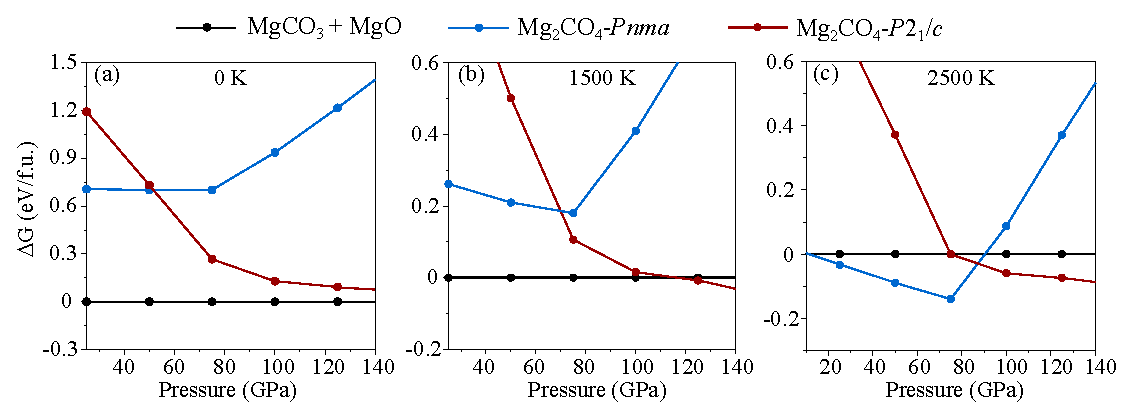
\includegraphics[width=\textwidth]{transition} \centering
	\caption{The relative Gibbs free energies as function of pressure for Mg$_2$CO$_4$=MgCO$_3$+MgO reaction at 0 K (a), 1500 K (b), and 2500 K (c).} \label{gibbs}
\end{figure}


\begin{figure}[H]
	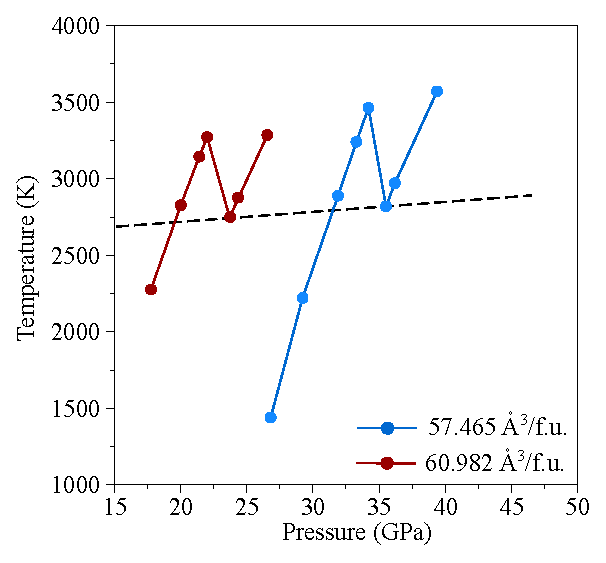
\includegraphics[width=0.6\textwidth]{Zcurve} \centering
	\caption{The Z isochores for Mg$_2$CO$_4$-$Pnma$ at volumes 53.252 \AA{$^3$}/f.u., 57.465 \AA{$^3$}/f.u. and 60.982 \AA{$^3$}/f.u. shown by blue and red lines, respectively.} \label{Zcurve}
\end{figure}

	\begin{table}[H]
	\caption{Calculated elastic constants $C_{ij}$ (GPa) of MgCO$_3$-$R\bar{3}c$ and Mg$_2$CO$_4$-$Pnma$ at 50 GPa and 0 K.} \label{elastic_const} \vspace{2mm} 
	\begin{tabular}{l*{10}{l}}
		\hline \hline
Phase	&	$C_{11}$	&	$C_{12}$	&	$C_{13}$	&	$C_{22}$	&	$C_{23}$	&	$C_{33}$	&	$C_{44}$	&	$C_{55}$	&	$C_{66}$	\\
\hline
Mg$_2$CO$_4$-$Pnma$	&	375.9	&	272.6	&	234.5	&	497	&	253.4	&	572.9	&	170.6	&	161.3	&	124.4	\\                                                                                              
MgCO$_3$-$R\bar{3}c$	&	543.9	&	239.5	&	230.6	&	543.9	&	230.6	&	352.4	&	122.4	&	122.4	&	152.3	\\

		\hline \hline
	\end{tabular}
\end{table}

	\begin{table}[H]
	\caption{Calculated density $\rho$ (kg/m$^3$), bulk modulus $B$ (GPa), shear modulus $G$ (GPa), compression $V_p$ (km/s) and shear $V_s$ (km/s) velocities, compression anisotropy $A_B$, shear anisotropy $A_G$, and universal anisotropy $A^U$ indexes of Mg$_2$CO$_4$-$Pnma$ and MgCO$_3$-$R\bar{3}c$ at 50 GPa and 0 K.} \vspace{2mm} \label{moduli}
		\begin{tabular}{l*{9}{l}}
			\hline \hline
					
			Phase	& $\rho$	& B &	G	& $V_p$&  $V_s$ &	$A_B$	&	$A_G$	&	$A^U$	\\
			\hline
			Mg$_2$CO$_4$-$Pnma$	& 3951.72 &	324.3	&	131.3	& 11.24  & 5.77 &	0.0165	&	0.0425	&	0.4772	\\
			MgCO$_3$-$R\bar{3}c$ & 3798.67 &	307.8	&	125.9	& 11.19 & 5.76	&   0.0256	&	0.0226	&	0.2838	\\
			
			\hline \hline
	\end{tabular}
\end{table}


\bibliographystyle{CGD}
\bibliography{sup_lib}

\section*{Crystallographic information files for the predicted structures}

%! Добавьте сюда, пожалуйста, цифы для Pnma и P21/c

\end{document}
